\documentclass[aspectratio=169,11pt]{beamer}
\usepackage[utf8]{inputenc}
\usepackage[T1]{fontenc}
\usepackage[norsk]{babel}
\usepackage{lmodern,booktabs,tikz}
\usetikzlibrary{arrows.meta,positioning}
\definecolor{adaptive}{HTML}{31105C}
\setbeamercolor{structure}{fg=adaptive}
\setbeamercolor{frametitle}{fg=white,bg=adaptive}
\setbeamertemplate{navigation symbols}{}
\setbeamertemplate{footline}[frame number]
\setbeamersize{text margin left=10mm,text margin right=10mm}
\title{ADAptive}
\subtitle{Autonom Mecanum-bil i Ada\\Arbeidsutkast: integrasjon og feilrespons}
\author{Nicolay Olafsen \and Jacob Hellumstand Utengen}
\institute{VE3140 -- Intelligente sanntidssystemer, USN}
\date{2. november 2026}
\begin{document}
\begin{frame}
\titlepage
\end{frame}

\begin{frame}{Problem og målbar demonstrasjon}
Hvordan kan micro:bit V2 styre bilen autonomt og reagere på hindringer
innenfor dokumenterte tidskrav?
\vspace{6mm}
\begin{enumerate}
\item Kjøre frem ved gyldige målinger og tilstrekkelig klaring.
\item Stoppe ved hindring, ukjent måling eller stoppforespørsel.
\item Skanne, velge en klarert sving og kontrollere omgivelsene på nytt.
\end{enumerate}
\vspace{5mm}
\alert{Full autonom gulvkjøring er fortsatt ikke fysisk validert.}
\end{frame}

\begin{frame}{Pi-en støtter utviklingen -- micro:biten styrer bilen}
\centering
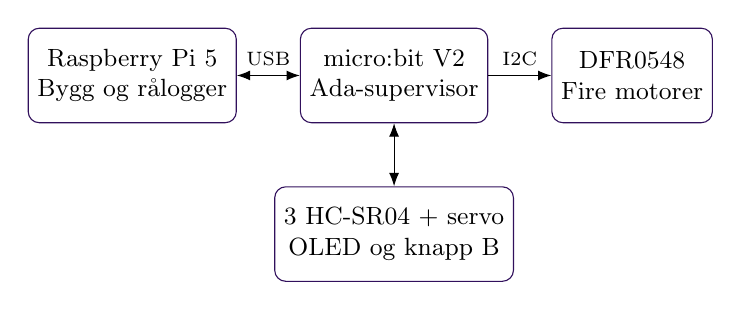
\begin{tikzpicture}[node distance=8mm,>=Latex,
 box/.style={draw=adaptive,rounded corners,align=center,minimum height=12mm,font=\small}]
\node[box] (pi) {Raspberry Pi 5\\Bygg og rålogger};
\node[box,right=of pi] (mb) {micro:bit V2\\Ada-supervisor};
\node[box,right=of mb] (motor) {DFR0548\\Fire motorer};
\node[box,below=of mb] (sensor) {3 HC-SR04 + servo\\OLED og knapp B};
\draw[<->] (pi)--node[above,font=\scriptsize]{USB}(mb);
\draw[->] (mb)--node[above,font=\scriptsize]{I2C}(motor);
\draw[<->] (mb)--(sensor);
\end{tikzpicture}
\vspace{5mm}
\begin{itemize}
\item Ada-kjernen kjører fortsatt sekvensielt; stoppflagget settes fra avbrudd.
\item Ingen antakelse om sanntidsgaranti fra Linux eller USB.
\item Motorstrøm isoleres før USB kobles til ukjent firmware.
\end{itemize}
\end{frame}

\begin{frame}{Normal kontroll og feil har hver sin betydning}
\begin{columns}[T]
\column{.49\textwidth}
\textbf{Normal kontrollflyt}
\begin{itemize}
\item Stopp $\rightarrow$ kontroller $\rightarrow$ kjør.
\item Hindring $\rightarrow$ stopp $\rightarrow$ skann.
\item Skann $\rightarrow$ trygg sving $\rightarrow$ ny kontroll.
\item Ugyldig sensor betyr ukjent avstand.
\end{itemize}
\column{.49\textwidth}
\textbf{Eksepsjonelle feil}
\begin{itemize}
\item Motorbuss avviser sending.
\item Ufullstendig motorinitialisering.
\item Ugyldig servovinkel.
\item Stoppknapp kunne ikke registreres.
\end{itemize}
\end{columns}
\vspace{6mm}
\alert{Ingen automatisk gjenstart etter en latchet feil.}
\end{frame}

\begin{frame}{Exception-responsen er testbar}
\begin{enumerate}
\item Bevar den opprinnelige feiltypen.
\item Sett stoppflagget før videre arbeid.
\item Forsøk én begrenset stoppoperasjon.
\item Skill mellom anerkjent kommando og mislykket sending.
\item Logg feil og eventuell sekundær stoppfeil.
\end{enumerate}
\vspace{6mm}
En loggerfeil utløser ikke ny kjøring. Et stopp som bussen har akseptert,
beviser ikke at hjulene står stille. Fysisk strømfrakobling må være mulig.
\end{frame}

\begin{frame}{En konkret oppstartsforbedring}
\textbf{Risiko:} Et motorstyrekort som fortsatt har strøm kan beholde gamle
PWM-verdier når micro:biten starter på nytt.
\vspace{5mm}
\begin{itemize}
\item Motorutgangene settes nå til FULL\_OFF før oscillatorens oppvåkning.
\item Ved ukjent auto-increment adresseres alle åtte motorkanaler enkeltvis.
\item Motor og OLED beholder én initialisering av felles ekstern I2C-buss.
\item Feilloggen inkluderer enhetsadresse, register og I2C-status.
\end{itemize}
\vspace{5mm}
\alert{Verifisert mot simulert buss. Den tidligere fysiske oppstartsfeilen
må fortsatt lokaliseres og testes på bilen.}
\end{frame}

\begin{frame}{Responstid må følge den faktiske arkitekturen}
\[
 R_{\mathrm{reaksjon}} = T_{\text{til neste måling}}
   + C_{\mathrm{sensor}} + C_{\mathrm{beslutning}} + C_{\mathrm{stopp}}
\]
\begin{itemize}
\item I2C-timeoutparameter: 20 ms per skriving.
\item Ukjent oppsett: opptil åtte stopptransaksjoner, samlet budsjett 160 ms.
\item Schedulerbidrag og fysisk bremsing kommer i tillegg.
\item Maksimal observert kjøretid er ikke bevist WCET.
\end{itemize}
\vspace{4mm}
\alert{Periodiske applikasjonstasks og full RTA er neste arkitekturfase.}
\end{frame}

\begin{frame}{Matematikken skal påvirke bilen}
\[
 d_{\mathrm{stopp}}=v\,t_{\mathrm{reaksjon}}+\frac{v^2}{2a_b}+d_{\mathrm{margin}}
\]
\begin{itemize}
\item Fart og bremseretardasjon må måles; PWM er ingen fartsmåling.
\item Pulsvarighet gir avstandsestimat med usikkerhet og gyldighetskontroll.
\item Klaring må ta hensyn til chassis, sensorgeometri og svingbevegelse.
\end{itemize}
\vspace{5mm}
Historiske 60 cm-forsøk ga 480/480 gyldige venstremålinger og middel
57,108 cm. Dette viser repeterbarhet i oppsettet og et avvik som krever
flerpunktkalibrering; det beviser ikke kollisjonssikkerhet.
\end{frame}

\begin{frame}{Hva er faktisk testet?}
\small
\begin{tabular}{@{}p{.42\textwidth}p{.49\textwidth}@{}}\toprule
Kontroll & Status 2.11.2026\\\midrule
Native Ada-kontroller & 1857 består; 104 nye feil-/motorkontroller\\
Python-tester & 35 består; seks nye for passiv USB-logging\\
ARM-bygg & Hovedprogram, diagnostikk V2 og GPIO V3 består\\
Fysisk bil i denne økten & Ingen tilkoblet micro:bit, ingen flashing eller kjøring\\
Formell verifikasjon / deadlines & Ingen nye bevis; fysiske tidsmålinger gjenstår\\\bottomrule
\end{tabular}\par
\vspace{5mm}
Feilinjeksjon omfatter alle tolv skrivepunkter i oppstarten, stopp under
motorsending, sekundær stoppfeil og loggerfeil.
\end{frame}

\begin{frame}{Neste demonstrasjon og ferdigstilling}
\begin{enumerate}
\item USB-identifikasjon og oppstartslogg med motorstrøm isolert.
\item Stasjonære, oppmålte sensortester og løsning av fysisk I2C-feil.
\item Bekreft begge svingretninger med løftede hjul.
\item Mål lavfartskjøring, reaksjonstid og faktisk stopplengde.
\item Gjenta autonom sekvens med rålogg og video.
\end{enumerate}
\vspace{5mm}
Før innlevering: kontroller pensum og vurderingskriterier, komprimer
hovedrapporten til anbefalt omfang og dokumenter gruppens egne forklaringer,
arbeidsfordeling og KI-bruk.\par
\vspace{4mm}
\tiny Kilder: Ada 2022 RM 11.4, AdaCore runtime-dokumentasjon, NXP PCA9685
og micro:bit-stiftelsens USB-veiledning. Se rapportens bibliografi.
\end{frame}
\end{document}
